% This file was created with tikzplotlib v0.9.12.
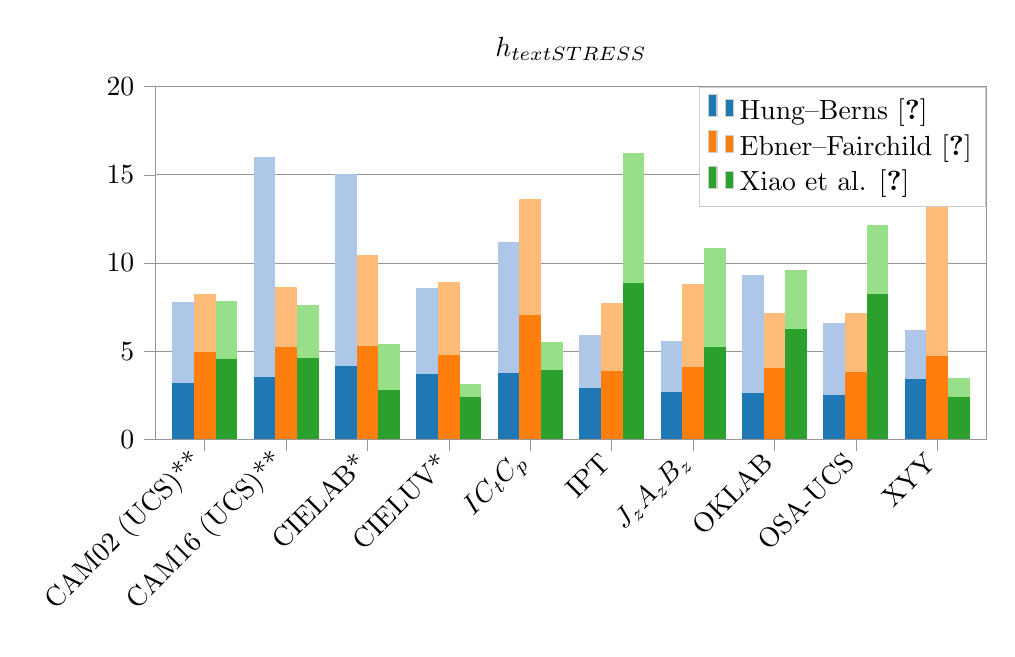
\begin{tikzpicture}

\definecolor{color0}{rgb}{0.12156862745098,0.466666666666667,0.705882352941177}
\definecolor{color1}{rgb}{0.682352941176471,0.780392156862745,0.909803921568627}
\definecolor{color2}{rgb}{1,0.498039215686275,0.0549019607843137}
\definecolor{color3}{rgb}{1,0.733333333333333,0.470588235294118}
\definecolor{color4}{rgb}{0.172549019607843,0.627450980392157,0.172549019607843}
\definecolor{color5}{rgb}{0.596078431372549,0.874509803921569,0.541176470588235}

\begin{axis}[
axis line style={white!58.8235294117647!black},
height=0.5\textwidth,
legend cell align={left},
legend style={fill opacity=1, draw opacity=1, text opacity=1, at={(1,1)}, draw=white!80!black},
tick align=outside,
tick pos=left,
title={\(\displaystyle h_{text{STRESS}}\)},
width=\textwidth,
x grid style={white!58.8235294117647!black},
xmin=-0.6, xmax=9.6,
xtick style={color=white!58.8235294117647!black},
xtick={0,1,2,3,4,5,6,7,8,9},
xticklabel style={rotate=45.0,anchor=east},
xticklabels={
  CAM02 (UCS)**,
  CAM16 (UCS)**,
  CIELAB*,
  CIELUV*,
  \(\displaystyle IC_tC_p\),
  IPT,
  \(\displaystyle J_zA_zB_z\),
  OKLAB,
  OSA-UCS,
  XYY
},
y grid style={white!58.8235294117647!black},
ymajorgrids,
ymin=0, ymax=20,
ytick style={color=white!58.8235294117647!black},
ytick={0,5,10,15,20}
]
\draw[draw=none,fill=color0] (axis cs:-0.4,0) rectangle (axis cs:-0.133333333333333,3.18845620008038);
\addlegendimage{ybar,ybar legend,draw=none,fill=color0}
\addlegendentry{Hung--Berns \cite{hung}}

\draw[draw=none,fill=color0] (axis cs:0.6,0) rectangle (axis cs:0.866666666666667,3.52855078191527);
\draw[draw=none,fill=color0] (axis cs:1.6,0) rectangle (axis cs:1.86666666666667,4.14821469192855);
\draw[draw=none,fill=color0] (axis cs:2.6,0) rectangle (axis cs:2.86666666666667,3.69928776179375);
\draw[draw=none,fill=color0] (axis cs:3.6,0) rectangle (axis cs:3.86666666666667,3.79577398935562);
\draw[draw=none,fill=color0] (axis cs:4.6,0) rectangle (axis cs:4.86666666666667,2.92119683105357);
\draw[draw=none,fill=color0] (axis cs:5.6,0) rectangle (axis cs:5.86666666666667,2.68536426894408);
\draw[draw=none,fill=color0] (axis cs:6.6,0) rectangle (axis cs:6.86666666666667,2.63371950519243);
\draw[draw=none,fill=color0] (axis cs:7.6,0) rectangle (axis cs:7.86666666666667,2.49530998013144);
\draw[draw=none,fill=color0] (axis cs:8.6,0) rectangle (axis cs:8.86666666666667,3.44018748653443);
\draw[draw=none,fill=color1] (axis cs:-0.4,3.18845620008038) rectangle (axis cs:-0.133333333333333,7.77803913385343);
\draw[draw=none,fill=color1] (axis cs:0.6,3.52855078191527) rectangle (axis cs:0.866666666666667,16.0323471051899);
\draw[draw=none,fill=color1] (axis cs:1.6,4.14821469192855) rectangle (axis cs:1.86666666666667,15.0311575636155);
\draw[draw=none,fill=color1] (axis cs:2.6,3.69928776179375) rectangle (axis cs:2.86666666666667,8.56391940890914);
\draw[draw=none,fill=color1] (axis cs:3.6,3.79577398935562) rectangle (axis cs:3.86666666666667,11.1890830346538);
\draw[draw=none,fill=color1] (axis cs:4.6,2.92119683105357) rectangle (axis cs:4.86666666666667,5.89478443004318);
\draw[draw=none,fill=color1] (axis cs:5.6,2.68536426894408) rectangle (axis cs:5.86666666666667,5.55970441646704);
\draw[draw=none,fill=color1] (axis cs:6.6,2.63371950519243) rectangle (axis cs:6.86666666666667,9.31997777958701);
\draw[draw=none,fill=color1] (axis cs:7.6,2.49530998013144) rectangle (axis cs:7.86666666666667,6.59231944961339);
\draw[draw=none,fill=color1] (axis cs:8.6,3.44018748653443) rectangle (axis cs:8.86666666666667,6.18717018996993);
\draw[draw=none,fill=color2] (axis cs:-0.133333333333333,0) rectangle (axis cs:0.133333333333333,4.96820230766771);
\addlegendimage{ybar,ybar legend,draw=none,fill=color2}
\addlegendentry{Ebner--Fairchild \cite{ebner}}

\draw[draw=none,fill=color2] (axis cs:0.866666666666667,0) rectangle (axis cs:1.13333333333333,5.25888517471055);
\draw[draw=none,fill=color2] (axis cs:1.86666666666667,0) rectangle (axis cs:2.13333333333333,5.29206832728103);
\draw[draw=none,fill=color2] (axis cs:2.86666666666667,0) rectangle (axis cs:3.13333333333333,4.81360584972163);
\draw[draw=none,fill=color2] (axis cs:3.86666666666667,0) rectangle (axis cs:4.13333333333333,7.04859738515829);
\draw[draw=none,fill=color2] (axis cs:4.86666666666667,0) rectangle (axis cs:5.13333333333333,3.8585452834895);
\draw[draw=none,fill=color2] (axis cs:5.86666666666667,0) rectangle (axis cs:6.13333333333333,4.11463844120849);
\draw[draw=none,fill=color2] (axis cs:6.86666666666667,0) rectangle (axis cs:7.13333333333333,4.05730886560147);
\draw[draw=none,fill=color2] (axis cs:7.86666666666667,0) rectangle (axis cs:8.13333333333333,3.81297237590754);
\draw[draw=none,fill=color2] (axis cs:8.86666666666667,0) rectangle (axis cs:9.13333333333333,4.75045818919245);
\draw[draw=none,fill=color3] (axis cs:-0.133333333333333,4.96820230766771) rectangle (axis cs:0.133333333333333,8.22072308329214);
\draw[draw=none,fill=color3] (axis cs:0.866666666666667,5.25888517471055) rectangle (axis cs:1.13333333333333,8.66022068747131);
\draw[draw=none,fill=color3] (axis cs:1.86666666666667,5.29206832728103) rectangle (axis cs:2.13333333333333,10.4569873793138);
\draw[draw=none,fill=color3] (axis cs:2.86666666666667,4.81360584972163) rectangle (axis cs:3.13333333333333,8.91448406046236);
\draw[draw=none,fill=color3] (axis cs:3.86666666666667,7.04859738515829) rectangle (axis cs:4.13333333333333,13.6280487760657);
\draw[draw=none,fill=color3] (axis cs:4.86666666666667,3.8585452834895) rectangle (axis cs:5.13333333333333,7.72233957150083);
\draw[draw=none,fill=color3] (axis cs:5.86666666666667,4.11463844120849) rectangle (axis cs:6.13333333333333,8.80555808427234);
\draw[draw=none,fill=color3] (axis cs:6.86666666666667,4.05730886560147) rectangle (axis cs:7.13333333333333,7.16171792324175);
\draw[draw=none,fill=color3] (axis cs:7.86666666666667,3.81297237590754) rectangle (axis cs:8.13333333333333,7.17861133082468);
\draw[draw=none,fill=color3] (axis cs:8.86666666666667,4.75045818919245) rectangle (axis cs:9.13333333333333,13.4354916910975);
\draw[draw=none,fill=color4] (axis cs:0.133333333333333,0) rectangle (axis cs:0.4,4.58825706817218);
\addlegendimage{ybar,ybar legend,draw=none,fill=color4}
\addlegendentry{Xiao et al. \cite{xiao}}

\draw[draw=none,fill=color4] (axis cs:1.13333333333333,0) rectangle (axis cs:1.4,4.62695701852859);
\draw[draw=none,fill=color4] (axis cs:2.13333333333333,0) rectangle (axis cs:2.4,2.78836260423616);
\draw[draw=none,fill=color4] (axis cs:3.13333333333333,0) rectangle (axis cs:3.4,2.38128547870168);
\draw[draw=none,fill=color4] (axis cs:4.13333333333333,0) rectangle (axis cs:4.4,3.92409485524028);
\draw[draw=none,fill=color4] (axis cs:5.13333333333333,0) rectangle (axis cs:5.4,8.85387808189672);
\draw[draw=none,fill=color4] (axis cs:6.13333333333333,0) rectangle (axis cs:6.4,5.2305294695945);
\draw[draw=none,fill=color4] (axis cs:7.13333333333333,0) rectangle (axis cs:7.4,6.25638644449191);
\draw[draw=none,fill=color4] (axis cs:8.13333333333333,0) rectangle (axis cs:8.4,8.22761086694145);
\draw[draw=none,fill=color4] (axis cs:9.13333333333333,0) rectangle (axis cs:9.4,2.3985002202066);
\draw[draw=none,fill=color5] (axis cs:0.133333333333333,4.58825706817218) rectangle (axis cs:0.4,7.8366298874709);
\draw[draw=none,fill=color5] (axis cs:1.13333333333333,4.62695701852859) rectangle (axis cs:1.4,7.63990114805117);
\draw[draw=none,fill=color5] (axis cs:2.13333333333333,2.78836260423616) rectangle (axis cs:2.4,5.41428572442929);
\draw[draw=none,fill=color5] (axis cs:3.13333333333333,2.38128547870168) rectangle (axis cs:3.4,3.13325181065191);
\draw[draw=none,fill=color5] (axis cs:4.13333333333333,3.92409485524028) rectangle (axis cs:4.4,5.52652985033793);
\draw[draw=none,fill=color5] (axis cs:5.13333333333333,8.85387808189672) rectangle (axis cs:5.4,16.2208566981952);
\draw[draw=none,fill=color5] (axis cs:6.13333333333333,5.2305294695945) rectangle (axis cs:6.4,10.855292125204);
\draw[draw=none,fill=color5] (axis cs:7.13333333333333,6.25638644449191) rectangle (axis cs:7.4,9.59481014620975);
\draw[draw=none,fill=color5] (axis cs:8.13333333333333,8.22761086694145) rectangle (axis cs:8.4,12.1368913781661);
\draw[draw=none,fill=color5] (axis cs:9.13333333333333,2.3985002202066) rectangle (axis cs:9.4,3.47049524917497);
\end{axis}

\end{tikzpicture}
